% Framework i*
\chapter{Framework i*, Variações e Ferramentas}
    \label{cap:framework}
    % intro
        Neste capítulo são apresentados os conceitos básicos necessários para o entendimento sobre a técnica de modelagem organizacional do framework i*, bem como os trabalhos baseados nessa técnica.
        Por fim, discute-se sobre algumas ferramentas de modelagem i* e/ou variações.
    % topics
        % framework i*
            Inicialmente, na seção \ref{cap:framework-sec:istar}, são apresentados os conceitos fundamentais do i* através dos seus dois componentes de modelagem e alguns dos meta-modelos existentes.
        % variacoes
            Na seção \ref{cap:framework-sec:variacoes}, mostra-se algumas variações ou extensões da proposta inicial do i* em \cite{yu1995modelling}.
        % ferramentas
            Em seguida, na seção \ref{cap:framework-sec:ferramentas}, comenta-se sobre a ferramentas OME, uma ferramenta que geram arquivos de entrada para a JGOOSE.
        % considerações finais do capítulo
            Por fim, na seção \ref{cap:framework-sec:conclusao}, são feitas algumas considerações finais do capítulo.
    %
    \section{O Framework i*}
        \label{cap:framework-sec:istar}
        % intro
            % o que é ?
                O framework i* (pronunciado ``i-star''
                        \footnote{O nome i*, pronunciado em inglês ``i-star'' faz referência ao conceito sobre uma intencionalidade distribuída. No Brasil, são comuns as pronúncias ``i-estrela'' e ``i-star''.}),
                    originalmente proposto por Yu \cite{yu1995modelling},
                é um framework de modelagem organizacional conceitual.
                Ou seja, ajuda no desenvolvimento de modelos que auxiliam a análise de sistemas sob uma visão estratégica e intencional de processos que envolvem vários participantes.

            % pra que server?
                O framework i* preocupa-se principalmente com a análise do contexto organizacional e social de um sistema.
                O sistema, nesse caso, não consiste somente em componentes técnicos, mas também de elementos humanos.
            % aplicações em várias áreas
                Como o framework i* é bastante flexível para representar situações envolvendo interações entre múltiplos participantes,
                esse framework pode ser utilizado para representar variados contextos organizacionais.

                A seguir, têm-se alguns contextos onde a modelagem i* vem sendo aplicada:
                    \begin{itemize}
                        \item[] \textbf{Engenharia de Requisitos}:
                            é uma das áreas de aplicações mais comuns do i*, principalmente nas fases iniciais do processo de engenharia de requisitos (\emph{Early Requirements})
                            \cite{yu1997towards} e \cite{maiden2004model};

                        \item[] \textbf{Modelagem de Negócio (Business Modeling)}:
                            estudos na área apresentaram o uso do i* para visualização explícita da intencionalidade por trás dos processos de negócios.
                            Isso ajuda a se obter um melhor entendimento sobre o trabalho, além de facilitar seu replanejamento
                            \cite{yu1996models} \cite{kolp2003organizational};

                        \item[] \textbf{Desenvolvimento Orientado à Objeto}:
                            em \cite{castro2000closing} e \cite{castro2001integrating}
                            utilizou-se da pUML (precise UML) \cite{evans1999core}
                            e da \emph{Object Constraint Language} (OCL) \cite{warmer2003object}
                            para tratar dos requisitos finais (\emph{Late Requirements}), além de usar o framework i* para os requisitos iniciais;

                        \item[] \textbf{Desenvolvimento Orientado à Agentes}:
                            em \cite{bresciani2004tropos} apresentou-se o uso de agentes com estrutura BDI (\emph{Believe, Desire and Intention}) \cite{rao1995bdi} para realizar análises na fase inicial de requisitos.
                            Já em \cite{bastos2004enhancing}, utilizou-se de Sistemas Multi-Agentes (SMA) para especificar a estrutura organizacional;

                        \item[] \textbf{Segurança, Confiabilidade e Privacidade}:
                            a modelagem i* pode ajudar a lidar com elementos de segurança, confiabilidade e privacidade, através do estudo dos conflitos de intenções de diferentes entidades sociais \cite{yu2001modelling};
                    \end{itemize}

            % orientado a agente/objetivo?
                Segundo \cite{yu2011social}, pode-se dizer que o i* é um framework de modelagem tanto orientado a agentes quanto orientado a objetivos, pois sua essência é realizada na combinação de agentes/atores e objetivos.
                Ambos os paradigmas, Orientação à Agentes \cite{mao2005organizational} e Orientação à Objetivos \cite{van2004goal}, têm apresentado bons resultados em contextos de modelagem organizacional, principalmente em modelagens da fase inicial (\emph{Early Requirements}) do processo de engenharia de requisitos. % TODO: cite?

            % como funciona?
                O i* é composto por dois components de modelagem: modelo de dependências estratégicas e modelo de razões estratégicas.
                Esses componentes auxiliam na representação, respectivamente, das dependências entre atores e dos detalhes por atrás das dependências de cada ator.
                É fundamental conhecer as notações e saber aplicar esses conceitos para se construir um bom modelo organizacional \cite{webster2005survey}.
                A seguir, são apresentados os conceitos e notações por trás dos modelos \cite{site2013iwiki}.

        \subsection{Modelo de Dependências Estratégicas}
            % intro
                O modelo de Dependência Estratégica (SD)\footnote{SD, do inglês Strategic Dependency},
                representa um conjunto de relacionamento estratégicos externos entre os atores organizacionais, formando uma rede de dependências.
                Fornece uma visão mais abstrata e ampla da organização, sem se preocupar com os detalhes (razões internas) por trás dessas dependências.

            \paragraph{Atores, Especializações e Fronteira}
                \begin{enumerate}[i.] % for capital roman numbers.
                    \item \textbf{Ator} pode ser definido como uma entidade (humana ou computacional) que age sobre o meio que está inserido para conquistar seus objetivos, exercitando seu \emph{know-how} \cite{yu1995modelling}. Atores podem ser vistos como uma referência genérica a qualquer unidade que se possa atribuir dependências intencionais. Os atores possuem relações de dependências com outros atores para um determinado fim. Quando existe uma necessidade de maiores detalhes sobre um modelo organizacional, atores podem ser diferenciados em três especializações: agentes, posições e papéis. A Figura \ref{fig:atores} exemplifica os tipos de atores, enquanto a Figura \ref{fig:atores-exemplo} apresenta um exemplo dos possíveis relacionamento entre os tipos de atores. A seguir, descreve-se esses tipos:
                    
                    \begin{figure}[h!]
                        \centering
                            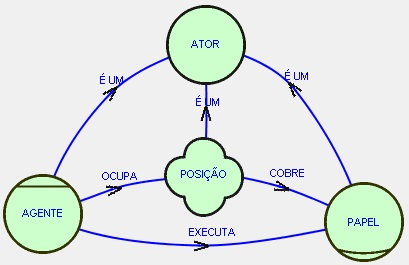
\includegraphics[scale=0.8]{Figuras/istar/atores.jpg}
                            \caption{Exemplo de relações entre atores \cite{santos2008istar}}
                            \label{fig:atores-exemplo}
                    \end{figure}

                    \begin{figure}[h!]
                        \centering
                            \subfigure[fig:ator:a][Ator]{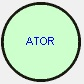
\includegraphics[scale=0.8]{Figuras/istar/ator.jpg}}
                            \subfigure[fig:ator:b][Agente]{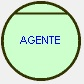
\includegraphics[scale=0.8]{Figuras/istar/ator-agente.jpg}}
                            \subfigure[fig:ator:c][Posição]{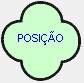
\includegraphics[scale=0.8]{Figuras/istar/ator-posicao.jpg}}
                            \subfigure[fig:ator:d][Papel]{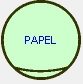
\includegraphics[scale=0.8]{Figuras/istar/ator-papel.jpg}}
                            \caption{Atores e especializações.}
                            \label{fig:atores}
                    \end{figure}
                    
                    %
                    \item \textbf{Agente} é a decomposição de um ator que possui manifestações físicas concretas. Refere-se tanto a humanos quanto a agentes de software ou hardware. Um agente possui dependências independentemente do papel que está executando. As características de um agente normalmente não são fáceis de se transferir para outros atores/agentes. São como experiências, habilidades ou, até mesmo, limitações físicas.
                    %
                    \item \textbf{Posição} representa uma abstração intermediária entre um agente e um papel. É o conjunto de papéis tipicamente executados por um agente, ou seja, representa uma posição dentro da organização onde o agente pode desempenhar várias funções (papéis). Diz-se que um agente ocupa uma posição e uma posição cobre um papel.
                    %
                    \item \textbf{Papel} é a caracterização abstrata do comportamento de um ator dentro de determinados contextos sociais ou domínio de informação. Essas características devem ser facilmente transferíveis a outro ator social. As dependências associadas a um papel são aplicáveis independentemente do agente que desempenha o papel.
                \end{enumerate}

            % actors associations
            \paragraph{Associações entre Atores:}
                As associações entre os atores são descritas através de links de associação (conforme a Figura \ref{fig:associations}.
                Essas associações podem ser de seis tipos:

                \begin{enumerate}[i.]
                    \item \textbf{\emph{IS PART OF}} (faz parte de) - Nessa associação cada papel, posição e agente pode ter sub-partes. Em \emph{IS PART OF} há dependências intencionais entre o todo e sua parte. Por exemplo, a dependência do todo sobre suas partes para manter a unidade na organização.

                    \item \textbf{\emph{ISA}} (é um) - Essa associação representa uma generalização, com um ator sendo um caso especializado de outro ator. Ambas, \emph{ISA} e \emph{IS PART OF}, podem ser aplicadas entre quaisquer duas instâncias do mesmo tipo de ator.
                    
                    \item \textbf{\emph{PLAYS}} (executa) - A associação plays é usada entre um agente e um papel, com um agente executando um papel. A identidade do agente que executa um papel não deverá ter efeito algum nas responsabilidades do papel ao qual está associado, e similarmente, aspectos de um agente deverão permanecer inalterados mesmo associados a um papel que este desempenha.
                    
                    \item \textbf{\emph{COVERS}} (cobre) - A associação covers é usada para descrever uma relação entre uma posição e os papéis que esta cobre.
                    
                    \item \textbf{\emph{OCCUPIES}} (ocupa) - Esta associação é usada para mostrar que um agente ocupa uma posição, ou seja, o ator executa todos os papéis que são cobertos pela posição que ele ocupa.
                    
                    \item \textbf{INS} - Esta associação é usada para representar uma \textbf{INS}tância específica de uma entidade mais geral. Por exemplo, quando se deseja representar um agente que é uma instanciação de outro agente.
                \end{enumerate}
                \begin{figure}[h!]
                    \centering
                        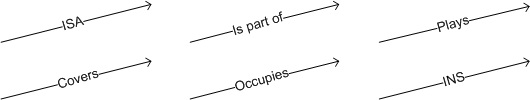
\includegraphics[width=0.8\linewidth]{Figuras/istar/actor-associations.jpg}
                        \caption{Tipos de associações entre atores \cite{site2013iwiki}.}
                        \label{fig:associations}
                \end{figure}

            % Elements
            \paragraph{Relação de Dependência}
                Uma relação de dependência pode ser deifinida como um acordo entre dois atores.
                Os elementos que compõe uma relação de dependência são:
                \begin{enumerate}[i.]
                    \item \emph{\textbf{Depender}}: é o ator dependente, ou seja, o ator que precisa que o acordo (\emph{Dependum}) seja realizado. Esse ator não se importa como o outro ator (\emph{Dependee}) irá satisfazer a necessidade da dependência.
                    \item \emph{\textbf{Dependum}}: é o elemento intermediário, objeto de questionamento e validação, da relação de dependência. % Ou seja, TODO
                    \item \emph{\textbf{Dependee}}: é o ator que tem a responsabilidade de satisfazer a relação de dependência.
                \end{enumerate}

                Dessa forma, pode-se classificar o tipo de uma relação de dependência com base em dos seguintes tipos de \emph{Dependum}:
                \begin{enumerate}[i.]
                    \item \textbf{Objetivo} (\emph{Goal}) - é uma declaração de afirmação sobre um certo estado do mundo. Deve ser de fácil verificação. O \emph{Dependee} é livre para tomar qualquer decisão para satisfazer o objetivo e é esperado que ele o faça. Não importa para o \emph{Depender} como o \emph{Dependee} irá alcançar esse objetivo.
                    %
                    \item \textbf{Tarefa} (\emph{Task}) - é uma atividade a ser realizada pelo \emph{Dependee}. Tarefas podem ser vistas com a realização de operações, processos e etc. Porém, não deve ser uma descrição passo-a-passo ou uma especificação completa de execução de uma rotina.
                    %
                    \item \textbf{Recurso} (\emph{Resource}) - é entidade (física ou informativa) a ser entregue para o \emph{Depender} pelo \emph{Dependee}. Satisfazendo-se esta dependência, o \emph{Depender} está habilitado a usar essa entidade como um recurso.
                    %
                    \item \textbf{Objetivo-Soft} (\emph{Softgoal}) - é semelhante ao Objetivo, porém os critérios de avaliação e verificação são mais subjetivos. O \emph{Depender} pode decidir sobre o que constitui a realização satisfatória do objetivo.
                \end{enumerate}
                % \begin{figure}[h!]
                %     \centering
                %         \includegraphics[width=0.7\linewidth]{Figuras/istar/dependency-links.jpg}
                %         \caption{Exemplo de Relação de Dependência (\emph{Dependder} -> \emph{Dependum} -> \emph{Dependee})}
                %         \label{fig:dependency-links}
                % \end{figure}
                % A Figura \ref{fig:dependency-links} apresenta alguns exemplos de relações de dependências.
            
            % Links (One side)
            \paragraph{Ligação de dependência}
                É uma estritamente a conexão entre os elementos de forma direcionada.
                Assim, pode-se ter somente duas opções de conexão: início no \emph{Depender}, fim no \emph{Dependum} e início no \emph{Dependum} e fim no \emph{Dependee}. Essa conexão é definida por um segmento contínuo, com a letra ``D'' sobrescrita, e direcionada da origem para o destino (conforme os exemplos da Figura \ref{fig:dependency}).
                % Assim, pode-se pensar na seguinte estrutura de nodos e ligações:
                %     1. \emph{Depender} (nodo); 2. Ligação de dependência (ligação); 3. \emph{Dependum} (nodo); 4. Ligação de dependência (ligação); 5. \emph{Dependee} (nodo).
                \begin{figure}[h!]
                    \centering
                        \subfigure[fig:dependency:empty][Ligação de Dependência.]{
\includegraphics[scale=1]{Figuras/istar/dependency-empty.jpg}}
                        \\
                        \subfigure[fig:dependency:depender-dependum][Ligação de Dependência: do \emph{Depender} para o \emph{Dependum}.]{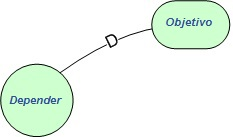
\includegraphics[width=0.4\linewidth]{Figuras/istar/dependency-depender-dependum.jpg}}
                        ~
                        \subfigure[fig:dependency:dependum-dependee][Ligação de Dependência: do \emph{Dependum} para o \emph{Dependee}.]{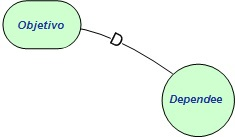
\includegraphics[width=0.4\linewidth]{Figuras/istar/dependency-dependum-dependee.jpg}}
                        \caption{Exemplos de ligação de dependência.}
                        \label{fig:dependency}
                \end{figure}
                
        % [end]
        \subsection{Modelos de Razões Estratégicas (SR)}
            % SR
                Já o modelo de Razões Estratégicas(SR)\footnote{SR, do inglês Strategic Rationale},
                representa os detalhes das razões internas que estão por trás das dependências dos atores.
                Com isso, é possível detalhar os interesses, preocupações e motivações específicas de um ator.
                Esse tipo de modelo também torna possível a avaliação de alteranativas em definições de processos.

                O modelo SR, além de poder conter todos os atores e dependências do SD, ``abre-se'' os Atores para se detalhar as dependências e expressar as razões.
                Ou seja, para os atores que precisam ser detalhados, é habilitado o limite da fronteira que deve estar visível e com espaço o suficiente para receber os elementos de dependência e/ou ligações internas. 
                Dessa forma, pode-se pensar nos elementos internos ao ator, ou seja, dentro da área de fronteira, como ``pertencentes'' ao ator.
                A seguir, são descritos os demais elementos de um modelo SR.

            \paragraph{Fronteira}
                Uma fronteira indica os limites intecionais de um determinado ator. Todos os elementos dentro dos limites de um ator, são explicitamente desejos ou pretenções desse ator. Uma fronteira é representada por um círculo tracejado e o elemento do ator dessa fronteira deve ser sobreposto a ela, ficando acima do tracejado (conforme a Figura \ref{fig:boundary}).

                \begin{figure}[h!]
                    \centering
                        \subfigure[fig:boundary:a][Fronteira Vazia]{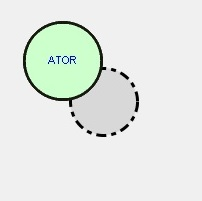
\includegraphics[width=0.3\linewidth]{Figuras/istar/boundary-empty.jpg}}
                        \subfigure[fig:boundary:b][Fronteira com elementos internos]{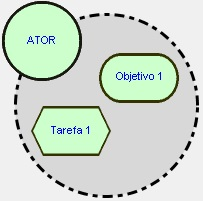
\includegraphics[width=0.3\linewidth]{Figuras/istar/boundary-non-empty.jpg}}
                        \caption{Exemplos de fronteira do ator.}
                        \label{fig:boundary}
                \end{figure}

            \paragraph{Ligação de meio-fim (\emph{means-end})}
                    % TODO: review.
                    É representada graficamente por uma seta direcionada ao nó fim, significando o meio para atingir um fim (objetivo, recurso, \emph{softgoal}, ou uma tarefa). A Figura \ref{fig:means-end} exemplifica este tipo de ligação.
                    \begin{figure}[h!]
                        \centering
                            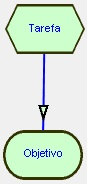
\includegraphics[scale=1]{Figuras/istar/means-end.jpg}
                            \caption{Exemplo de ligação meio-fim.}
                            \label{fig:means-end}
                    \end{figure}
                    %
                \paragraph{Ligação de decomposição (\emph{decomposition}):}
                    É responsável por detalhar e expressar da melhor como realizar uma determinada tarefa, através da decomposição em sub-elementos ligados  a  tarefa  principal (superior)  através  de  um  segmento  de  reta cortado.  Esses sub-elementos  podem  ser:  metas,  tarefas,  recursos  e  objetivos-soft.
                    \begin{figure}[h!]
                        \centering
                            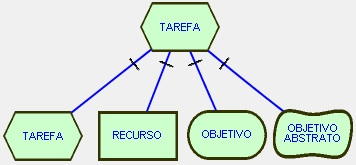
\includegraphics[scale=1]{Figuras/istar/decomposition.jpg}
                            \caption{Exemplo de ligação de decomposição.}
                            \label{fig:decomposition}
                    \end{figure}
                    %
                \paragraph{Ligações de Contribuição (\emph{contribution}):}
                    As ligações de contribuição são para ligar elementos à exclusivamente um objetivo-soft (\emph{softgoal}).
                    Essa ligação ajuda a modelar a forma como os elementos contribuem para a satisfação desse objetivo-soft (\emph{softgoal}).
                    Essas ligações de contribuição, ilustradas na Figura \ref{fig:contributions}, podem ser:
                    \begin{figure}[h!]
                        \centering
                            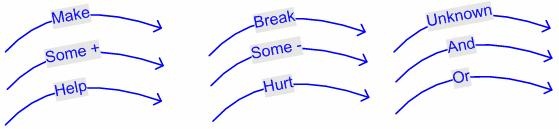
\includegraphics[scale=1]{Figuras/istar/contributions.jpg}
                            \caption{Ligações de contribuição \cite{site2013iwiki}.}
                            \label{fig:contributions}
                    \end{figure}
                    \begin{enumerate}[i.]
                        \item \textbf{\emph{Make}}: é uma contribuição positiva, suficientemente forte para satisfazer o objetivo-soft. 
                        \item \textbf{\emph{Some +}}: é uma contribuição positiva, mas cuja força de influência é desconhecida. Pode equivaler a um \emph{make} ou a um \emph{help}.
                        \item \textbf{\emph{Help}}: é uma contribuição positiva fraca, pois não é suficiente para que ela sozinha satisfaça o objetivo-soft.
                        \item \textbf{\emph{Unknown}}: é uma contribuição cuja influência é desconhecida. 
                        \item \textbf{\emph{Hurt}}: é uma contribuição negativa fraca, porém não é suficiente para que ela sozinha recuse a  satisfação de um objetivo-soft.
                        \item \textbf{\emph{Some -}}: é uma contribuição negativa, mas a força de sua influência é desconhecida. Pode equivaler a um \emph{hurt} ou a um \emph{break}.
                        \item \textbf{\emph{Break}}: é uma contribuição negativa, suficientemente forte para rejeitar a satisfação do objetivo-soft.
                        \item \textbf{\emph{Or}}: é uma contribuição onde o objetivo-soft é satisfeito se algum dos descendentes for satisfeitos. 
                        \item \textbf{\emph{And}}: é uma contribuição onde o objetivo-soft é satisfeito se todos os descendentes forem satisfeitos.
                    \end{enumerate}
                
        % [end]
        % \subsection{Diretrizes i* Wiki}
            %     % intro sobre as diretrizes
            %     No wiki do i* \cite{site2013iwiki} são apresentadas

            %     % TODO: reescrever
            %     As diretrizes são classificadas quanto ao nível:
            %         - iniciante: assume-se que o ?modelador? está tendo o primeiro contato com o framework de modelagem i*.
            %         - intermediário: 
            %         - avançado

            %     Quanto ao tipo:
            %         - conceito: esclarece questões sobre os fundamentos do framework
            %         - nomenclatura: como os atores, liks e elementos devem ser chamados? lida com questoes de cores e icones também.
            %         - notação: lida com a seleção adequada e uso da notação i* nos elementos, atores e links.
            %         - layout: lida com a disposição e organização dos modelos i* e o jeito que o conteúdo dos modelos 

        % [end]
    % [end]
    \section{Variações Baseadas no Framework i*}
        \label{cap:framework-sec:variacoes}
        % ITU-T = GRL + UCM.
        % yu95, i* wiki, GRL, Tropos, Aspectual i*, i*-c [6]
        % intro
            % Estudos da área já realizaram comparações entre as ferramentas.
            % Diferentes grupos de pesquisas que adotaram o framework i*.
            % Por vezes, o framework i* não atende todas as necessidades de um determinado grupo de pesquisadores.

        % exemplos
            % "O framework i* foi inicialmente proposto por [Yu 1995], mas hoje existem algumas extensões ou variações para sua versão original"
            % "Essas variações surgiram de diferentes grupos de pesquisa para atender ao propósito particular de cada um deles, e com isso surgiram diversas ferramentas de suporte."

        %problemas das variações i*
            % Conforme \cite{lucena2008}, as divergências quanto ao uso do i* podem causar:
            %     \begin{itemize}
            %         \item Divisão do esforço, ao passo que cada grupo de pesquisa irá focar no desenvolvimento de ferramentas de suporte ao seu próprio i*;
            %         \item Erros na semântica entre os projetistas e os leitores de um modelo particular do i*;
            %         \item Inibição da adoção/uso do i* por parte de novos usuários.
            %     \end{itemize}

        % vários estudos comparativos já foram realizados
            %http://istarwiki.org/tiki-index.php?page=i%2A+Modelling+Techniques&structure=i%2A+Wiki+Home
        % [end]
        \subsection{i* Wiki}
            % o que é?
                O i* Wiki, é um projeto criado com o intuito de reunir trabalhos relativos ao i*, de forma colaborativa
                    \cite{site2013iwiki} \cite{leuf2001wiki}.
                Com isso, a comunidade incentiva a colaboração dos usuários do framework, por meio de \emph{feedback} ou mesmo inserção de conteúdo em site oficial.
                Além disso, esses usuários podem sugerir alternativas ou extensões sintáticas e semânticas em relação a linguagem utilizada.
            
            % como funciona?
                Apesar da ampla visão que a comunidade pode ter com os trabalhos divulgados no site, a intenção é fornecer e evoluir uma única versão semântica do i*.
                Dessa forma, o i* Wiki funciona sobre duas versões do guia para o i* \cite{site2013iwiki}:
                    uma versão estável, servindo de referência para os usuários;
                    outra versão aberta a discussão, acessível aos usuários registrados no site e passível de comentários e sugestões individuais.
                Além disso, o site reúne um conjunto de Estudos de Casos, Publicações e Eventos relacionados a área de i*.
        % [end]

        \subsection{\emph{Goal-Oriented Requirements Language} (GRL)}
            A GRL é uma linguagem de apoio à modelagem orientada a agentes e objetivos.
            Assim como o i*, a GRL foca na modelagem dos relacionamentos estratégicos entre atores e seus objetivos.
            Pode-se pensar como uma alternativa que concentra recursos das metodologias NFR (\emph{Non-Functional Requirements}), i* e Tropos \cite{regev2005goals}.
            Outro ponto interessante é que a GRL é escalável, podendo se trabalhar com diferentes níveis de granularidade, em múltiplos diagramas ou visões de um mesmo modelo.

            Além disso, uma combinação da GRL com a \emph{Use Case Map} (UCM) deu origem a \emph{User Requirement Notation} (URN) - um padrão internacional do \emph{International  Telecommunication  Union} (ITU) para notação de requisitos de usuário.

        % [end]

        \subsection{Tropos}
            Tropos é um projeto que foi lançado em 2000 \cite{mylopoulos2001uml}, e visa apoiar a construção de sistemas de software orientados a agentes.
            O projeto reúne um grupo de autores de diversas Universidades no Brasil, Canadá, Bélgica, Alemanha, Itália, etc.
                % Tropos tem como objetivo o  desenvolvimento de sistemas de acordo com as reais necessidades de uma organização, buscando um melhor casamento entre o sistema e o ambiente em constante mudança.
            O processo de desenvolvimento segundo esta metodologia inicia com um estudo e elaboração de um modelo do ambiente no qual o sistema em desenvolvimento irá operar.
            Este modelo é refinado até que este represente o ambiente com o sistema em seu contexto.
            Cada modelo é descrito em termos dos atores observados no ambiente em modelagem, seus objetivos e relacionamentos.
            A metodologia Tropos oferece um framework que engloba as principais fases de desenvolvimento de software, com o apoio das seguintes atividades: Requisitos Iniciais, Requisitos Finais, Projeto Arquitetural e Projeto Detalhado.
        % [end]

    % [end]
    \section{Ferramenta OME }
        \label{cap:framework-sec:ferramentas}
        % intro
            Atualmente, existem várias ferramentas de modelagem i*.
            Pode-se encontrar mais de 20 ferramentas referenciadas no site do i* Wiki \cite{site2013iwiki}.
            % Ferramentas já foram comparadas. Listar trabalhos.
            Além disso, alguns trabalhos já realizaram comparações sobre ferramentas do framework i*,
                como em \cite{santos2008istar}(Tabela 6) e no site \cite{site2013iwiki}.

        % Pq só as duas?
            % Conforme foi comentado no Capítulo \ref{cap:introducao}, os arquivos de entrada aceitos pela JGOOSE devem estar no formato TELOS (.tel).
            % Além disso, conforme a apresentação da primeira versão da ferramenta em \cite{vicente2006}, as duas ferramentas que trabalham com esse formato são a OME e a OpenOME.
            % call next
            % Dessa forma, a OME e a OpenOME são apresentadas a seguir.

        % \subsection{OME}
            % intro
                O Ambiente de Modelagem Organizacional, tradução literal de OME - Organization Modelling Environment, é um editor gráfico de propósito geral para dar suporte à modelagem orientada a objetivo e/ou orientada a agentes.
                É uma aplicação Java para \emph{desktop} desenvolvida na Universidade de Toronto \cite{ome2013}.

            % about
                A ferramenta possui recursos que auxiliam o usuário no desenvolvimento e manipulação de modelos i* e NFR (\emph{Non-Functional Requirements}) \cite{chung2000non}.
                % history
                Em 2004, o desenvolvimento foi parado e seu código foi portado para a plataforma Eclipse \cite{eclipse}, dando origem a sua versão em código aberto chamda OpenOME \cite{horkoff2011openome}.
                % Aparentemente, a ferramenta parou na versão 3 (ou OME3) - mas ainda é mantida no site http://www.cs.toronto.edu/km/ome/.

                Apesar do seu desenvolvimento ter sido finalizado, ainda existem usuários da OME3.
                Além disso, a ferramenta possui um manual do usuário online (http://www.cs.toronto.edu/km/ome/docs/manual/manual.html) e é de fácil utilização. A maioria dos recursos i*, por exemplo, estão de acordo com \cite{yu1995modelling}.

            % exemplo final de tela:
                \begin{figure}[h!]
                    \centering
                        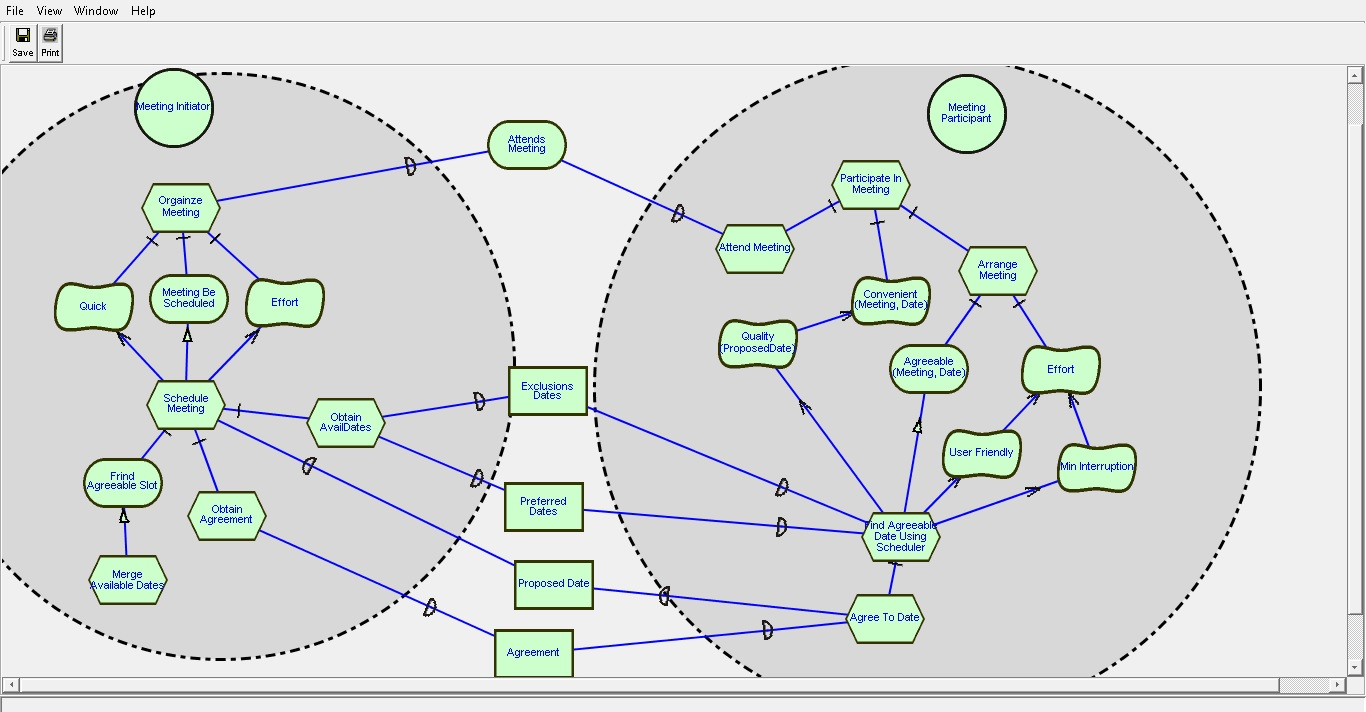
\includegraphics[width=0.8\linewidth]{Figuras/istar/tela-ome.jpg}
                        \caption{Exemplo de modelagem com a ferramenta OME3}
                        \label{fig:tela-ome}
                \end{figure}

                Como exemplo, têm-se na Figura \ref{fig:tela-ome} um dos modelos de exemplos já contidos na ferramenta OME3 junto à instalação (arquivo: ``Meeting-Schedule.tel'').
                Nessa tela, pode-se observar a barra de ferramentas (\emph{toolbar}) com as opções para criação dos elementos i*: atores, elementos de dependência, links  de  dependência, links  de  associação, etc.

                Cabe relembrar que essa ferramenta gera os modelos i* no formato TELOS, atualmente aceitos pela ferramenta JGOOSE.
                Além disso, considerando que a ferramenta apresenta problemas de instabilidade e seu processo de desenvolvimento foi descontinuado, acredita-se que a JGOOSE deva adotar uma nova solução para este fim.

    % [end]

    \section{iStarML}
        % intro
            Muitas ferramentas foram criadas com base nos conceitos do framework i* ou de variações desse \cite{cares2012towards} \cite{cares2011towards}.
            Isso acabou gerando modelos específicos para cada ferramenta, dificultando o intercâmbio de modelos entre essas ferramentas.
            Pensando nisso, foi desenvolvida a iStarML.
            Um meta-modelo baseado em XML (\emph{Extensible Markup Language}) usado para representar modelos i* \cite{cares2008istarml}.
            
            O principal objetivo desse meta-modelo é proporcionar um formato de intercâmbio entre os outros formatos de modelos do i*.
            Ou seja, a especificação iStarML deve suportar todas as outras definições e especificações dos modelos já propostos.
            Com isso, tudo o que se consegue especificar no formato TELOS, por exemplo, deve-se conseguir também no formato iStarML.

            Como prova de conceitos, foi realizado um estudo onde se aplicou o iStarML estritamente para fazer a interconexão entre duas ferramentas diferentes \cite{colomer2011model}.
            Nesse estudo, as ferramentas aplicadas foram jUCMNav \cite{kealey2006integrating} e a HiME \cite{lopez2009hime}.

            Porém, existe a preocupação sobre a real adoção da especificação iStarML. Como exemplo, tem-se a promessa da ferramenta OpenOME, que diz estar trabalhando para implementar rotinas de importação/exportação em iStarML \cite{horkoff2011openome} \cite{laue2011adding}.

            Conforme já mencionado no Capítulo \ref{cap:introducao}, é objetivo dessa pesquisa a implementação e adoção do iStarML como especificação do formato de arquivo padrão. Portanto, detalhes mais específicos sobre a linguagem iStarML serão feitas no Capítulo \ref{cap:proposta}.

    % [end]

    
    \section{Considerações Finais do Capítulo}
        \label{cap:framework-sec:conclusao}
        % o framework i* é importante (viu-se aplicações e benefícios em diversas áreas)
        %
            Neste Capítulo foram apresentados
                os conceitos gerais do framework i*, bem como as notaçãos da última versão do i* Wiki.
            Além disso,
                as variações do i* e seus respectivos meta-modelos, são estudados e analisados.
            Apesar das variações apresentadas, destaca-se a solução de intercâmbio entre diferentes formatos e ferramentas, iStarML.
            O iStarML foi adotado pelo editor proposto e será discutido melhor no Capítulo \ref{cap:proposta}.
    % [end]

% bibliography, just for auto-link in sublime text
% before compile main.tex, comment line below
% \bibliography{ref-unioeste,ref-commons,ref-books,ref-tecnologias,ref-istar}
